\chapter{Champ magnétique}

\minisec{Objectif}

\begin{enumerate}
  \item L'étudiant saura comment interagissent des pôles magnétiques à
    proximité.
  \item L'étudiant pourra appliquer la loi de Biot-Savart au calcul du champ
    magnétique produit par un fil infini.
\end{enumerate}


\section{Rappels sur les aimants}

\marginpar{
  Tremblay \S 8.1

  Lafrance \S 8.1
}

Un aimant a un pôle nord et un pôle sud. Le pôle nord est attiré vers le pôle
nord géographique. Le pôle sud de l'aimant est attiré vers le pôle sud
géographique.

Si on place deux aimants à proximité, les pôles de même type se repoussent, les
pôles opposés s'attirent. Par conséquent, le nord géographique est un pôle sud
magnétique.

Un aimant peut attirer certains matériaux non aimantés. C'est semblable à ce
qu'on observait entre une tige chargée et un matériau neutre.

Si on coupe un aimant en deux, chaque morceau possède un pôle nord et un pôle
sud. Il est impossible d'isoler un pôle. Autrement dit, il n'existe pas (selon
nos connaissances actuelles) de monopôles magnétiques.

Les aimants sont entourés d'un champ magnétique.

Le champ magnétique se mesure en tesla (\si{T}) ou en gauss (\SI{1}{G} =
\SI{1e-4}{T}). Le champ magnétique terrestre est de l'ordre de \SI{0.5}{G}. Le
champ magnétique produit par une machine d'imagerie par résonance magnétique
est de l'ordre de \SI{2}{T}.


\subsection{Lignes de champ magnétique}

Comme pour le champ électrique, on peut définir des lignes de champ magnétique.
Elles possèdent les propriétés suivantes:
\begin{itemize}
  \item champ magnétique tangent aux lignes de champ
  \item grandeur du champ magnétique proportionnel à la densité de lignes de
    champ
  \item à l'extérieur d'un aimant, les lignes de champ vont du pôle nord vers
    le pôle sud.
\end{itemize}
Puisqu'il n'y a pas de monopôle magnétique, les lignes de champ forment
toujours des courbes fermées.



\minisec{Question}

Quelle est l'orientation du champ magnétique à l'intérieur d'un aimant?


\begin{diapobox}
\minisec{Exercice}

Pour chacune des situations suivantes, déterminer si les deux objets
s'attirent, se repoussent, ou n'exercent aucune force l'un sur l'autre. (Note:
les lignes de champ ne sont tracées que partiellement.)

\begin{center}
  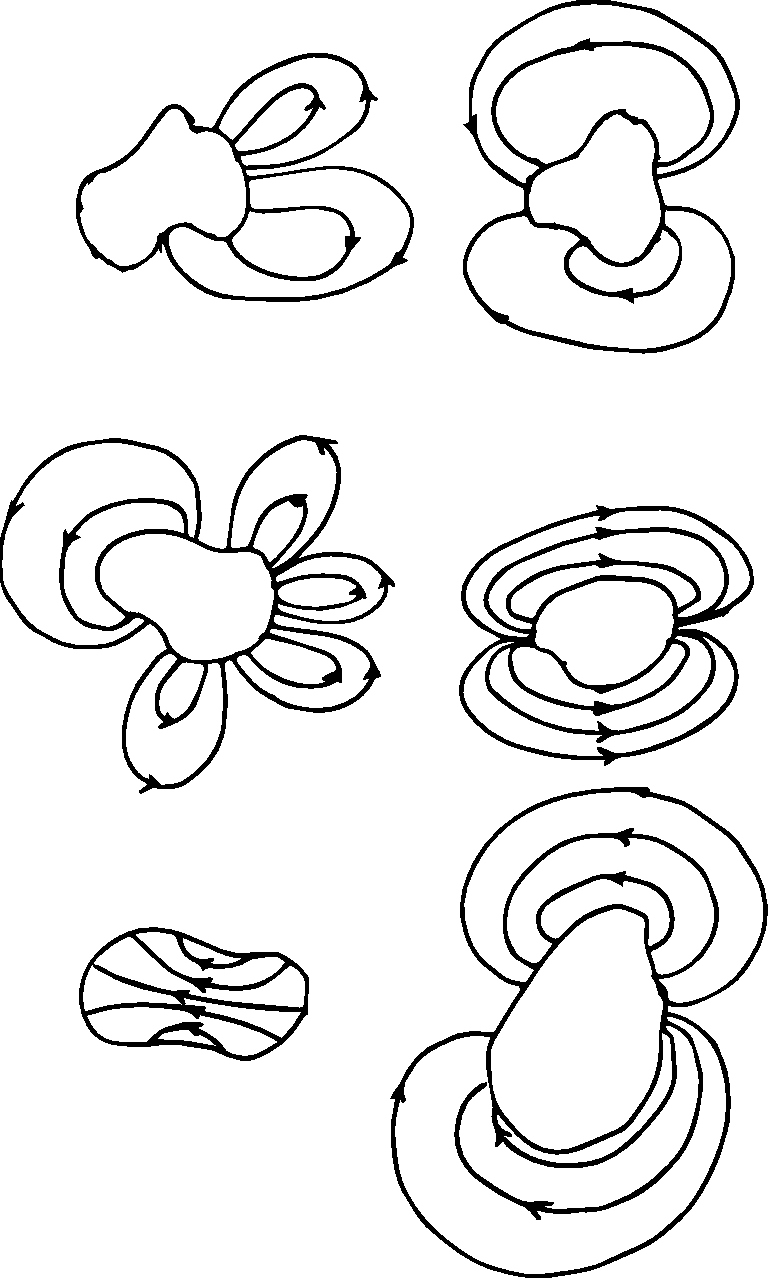
\includegraphics[scale=0.5]{08-champ-magnetique/figures/exercice-champ-magnetique1.pdf}
\end{center}

\end{diapobox}


\section{Source des champs magnétiques}

\marginnote{
  Lafrance \S 8.2
}

\minisec{Objectif}

\begin{enumerate}
  \item L'étudiant pourra appliquer la loi de Biot-Savart au calcul du champ
    magnétique produit par un fil infini.
\end{enumerate}


Démo avec un fil traversé d'un courant et une boussole. Montrer que la boussole
pointe toujours dans une direction tangente à un cercle centré sur le fil.

\begin{fondamentalbox}
  La source des champs magnétiques est le courant.
\end{fondamentalbox}

Les lignes de champ magnétique autour d'un long fil sont circulaire, centrées
sur le fil. L'orientation est obtenue à partir de la règle de la main droite.

\begin{diapobox}
  Quelle image illustre correctement le champ magnétique produit par le courant
  dans le fil?

  \begin{center}
    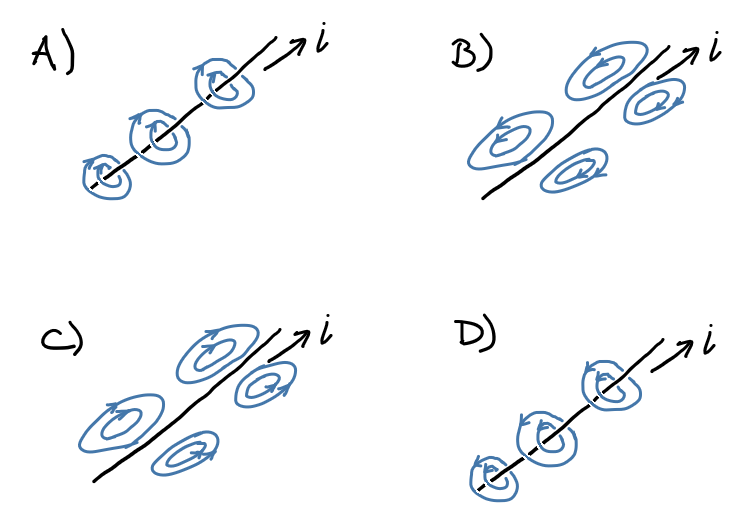
\includegraphics[scale=0.3]{08-champ-magnetique/figures/champ_fil_ex1.png}
  \end{center}

  \begin{center}
    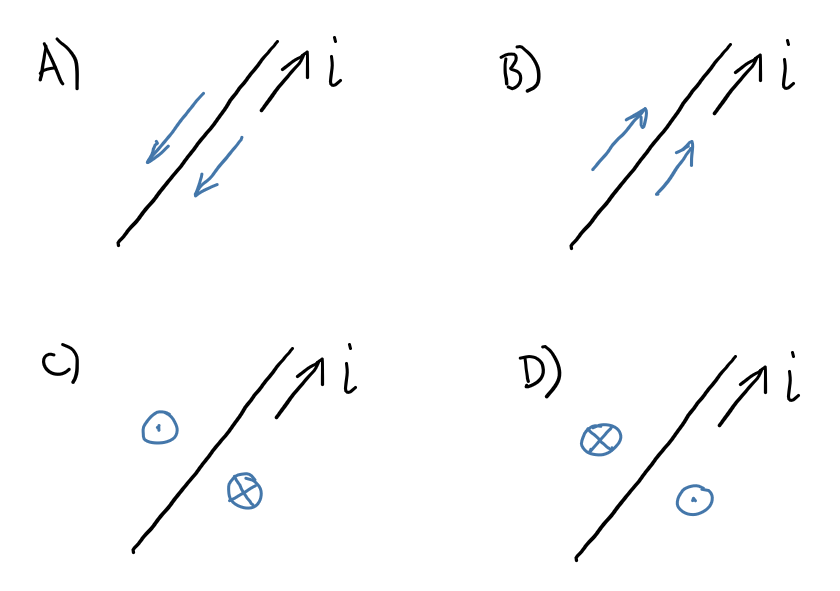
\includegraphics[scale=0.3]{08-champ-magnetique/figures/champ_fil_ex2.png}
  \end{center}
\end{diapobox}

\begin{diapobox}
  Quelle image illustre correctement le champ magnétique produit par le courant
  dans la boucle?

  \begin{center}
    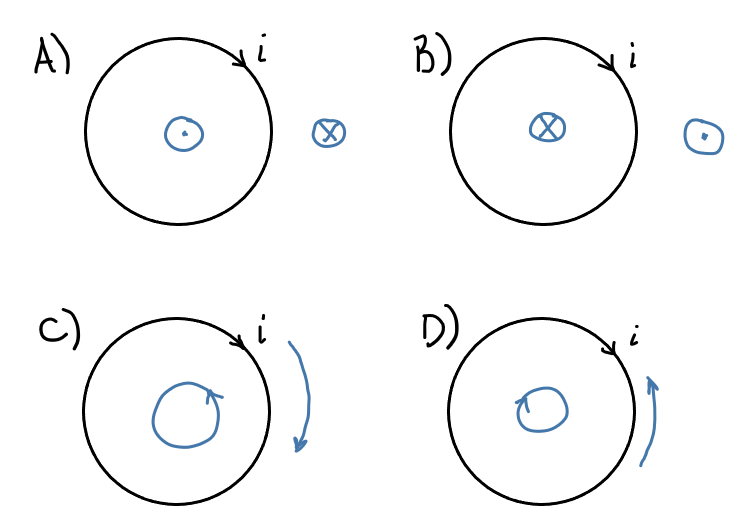
\includegraphics[scale=0.3]{08-champ-magnetique/figures/champ_boucle_ex1.png}
  \end{center}

  \begin{center}
    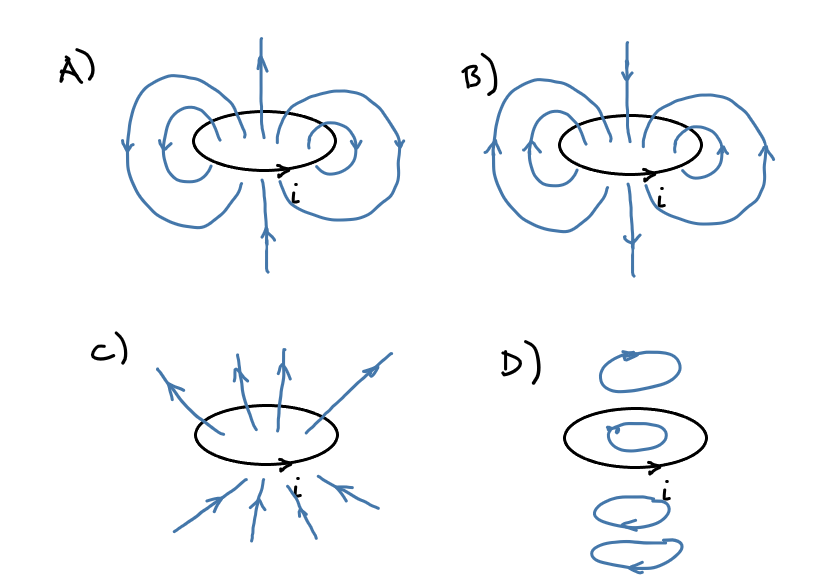
\includegraphics[scale=0.3]{08-champ-magnetique/figures/champ_boucle_ex2.png}
  \end{center}
\end{diapobox}

\begin{diapobox}
  \minisec{Champ magnétique d'un aimant}
  
  Quelle image illustre correctement les petites boucles de courant qui
  génèrent le champ d'un aimant?

  \begin{center}
    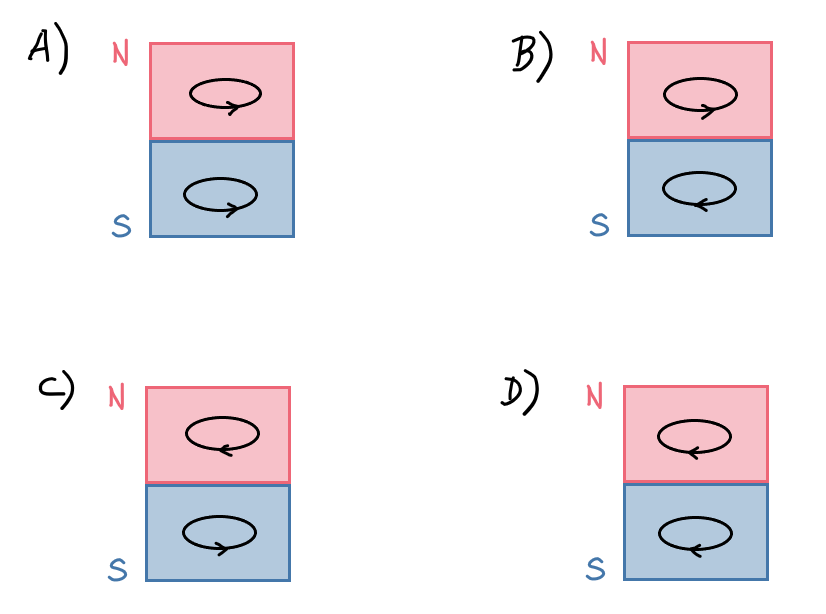
\includegraphics[scale=0.3]{08-champ-magnetique/figures/aimant_boucle.png}
  \end{center}

\end{diapobox}


\begin{fondamentalbox}
  \minisec{Loi de Biot-Savart}
  La loi de Biot-Savart est une formulation de ce qu'on vient
  d'observer.
  \marginnote{
  \begin{center}
    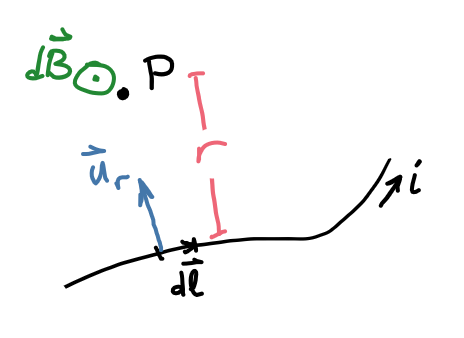
\includegraphics[scale=0.3]{08-champ-magnetique/figures/biot-savart.png}
  \end{center}
  }

  $$d\vB = \frac{\mu_0 I}{4\pi} \frac{d\vec{l} \times \vec{u}_r}{r^2} $$
  
  Le vecteur unitaire $\vec{u}_r$ va de la source du champ magnétique vers le
  point où le champ magnétique est calculé.
\end{fondamentalbox}

La constante $\mu_0$ s'appelle la \textbf{perméabilité du vide} (ou constante
magnétique) et vaut
$$\mu_0 = \SI{4\pi e-7}{Tm/A}$$


\begin{fondamentalbox}
  Le champ magnétique satisfait le principe de superposition, c'est-à-dire que
  le champ magnétique en un point est la somme vectorielle des champs produits
  par tous les courants à proximité.
\end{fondamentalbox}


\subsection*{Intermède mathématique : le produit vectoriel}

Le produit vectoriel entre deux vecteurs $\vu$ et $\vv$ est le vecteur de
grandeur
$$\abs{\vu \times \vv} = uv \sin\theta$$
orienté à \SI{90}{\degree} de $\vu$ et $\vv$ dans le sens donné par la règle de
la main droite.

\begin{diapobox}
  Classer les situations suivantes en ordre croissant de la grandeur du produit
  $\abs{\vu \times \vv}$.

  \begin{center}
    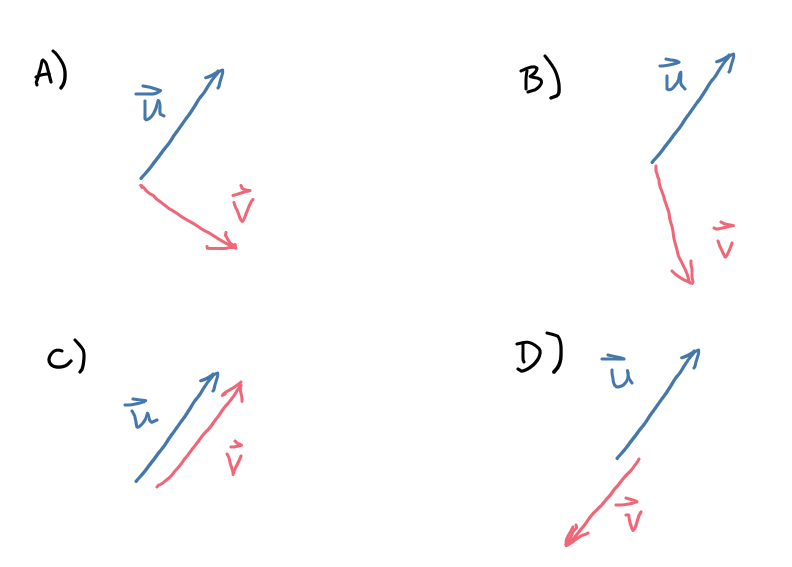
\includegraphics[scale=0.3]{08-champ-magnetique/figures/produit-vec_ex1.png}
  \end{center}
\end{diapobox}

Algébriquement, on peut calculer le produit vectoriel de $\vu =
\vecxyz{u_x}{u_y}{u_z}$ et $\vv = \vecxyz{v_x}{v_y}{v_z}$ comme suit
$$\vu \times \vv = \vecxyz{\left(u_y v_z - u_z v_y\right)}
                          {\left(u_z v_x - u_x v_z\right)}
                          {\left(u_x v_y - u_y v_x\right)}$$
Une approche complètement équivalente est de calculer le déterminant
$$
\vu \times \vv = \begin{vmatrix}
  \xhat  &  \yhat  &  \zhat  \\
  u_x    &  u_y    &  u_z    \\
  v_x    &  v_y    &  v_z
\end{vmatrix}
$$


\begin{diapobox}
\minisec{Exemple}

Calculer le produit vectoriel du vecteur $\vu = \vecxyz{3}{-2}{1}$ et du
vecteur $\vv$ dans le plan $xy$, de longueur $2$ et qui fait un angle de
\SI{30}{\degree} avec l'axe des $x$ positifs.
\end{diapobox}

\begin{reponsebox}
  On peut trouver les composantes de $\vv$ avec un peu de trigonométrie: $\vv =
  \vecxyz{\sqrt{3}}{1}{0}$. Ensuite, il suffit de calculer le produit
  \begin{align*}
    \vu \times \vv &= \begin{vmatrix}
      \xhat     &  \yhat  &  \zhat  \\
      3         &  -2     &  1      \\
      \sqrt{3}  &  1      &  0
    \end{vmatrix}  \\
  &= -\xhat + \sqrt{3} \yhat + (3 + 2 \sqrt{3})\zhat
  \end{align*}
\end{reponsebox}




\subsection*{Champ magnétique d'un fil infini}

Calculons le champ magnétique produit par un long fil rectiligne portant un
courant $i$, à une distance $a$ du centre du fil.
\marginnote{
  \begin{center}
    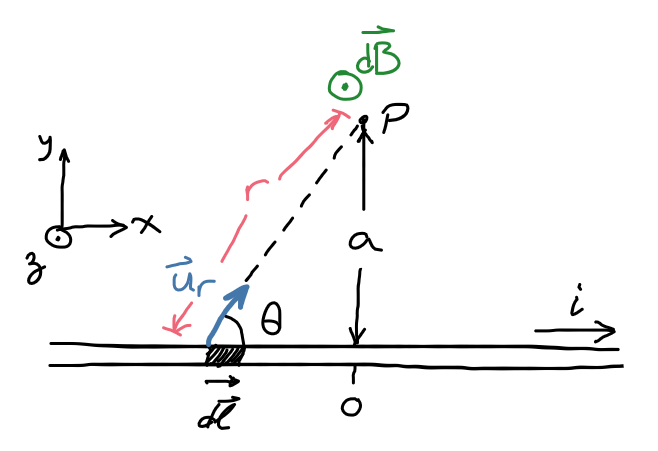
\includegraphics[scale=0.3]{08-champ-magnetique/figures/bs-champ-fil.png}
  \end{center}
}


Par la loi de Biot-Savart,
\begin{align*}
  d\vB &= \frac{\mu_0 i}{4\pi} \frac{d\vec{l} \times \vu_r}{r^2} \\
       &= \frac{\mu_0 i}{4\pi} \frac{dl \sin\theta \zhat}{r^2} \\
       &= \frac{\mu_0 i}{4\pi} \frac{dx a \zhat}{r^3}
\end{align*}
Par le principe de superposition, le champ total est obtenu en additionnant
les champs produits par tous les petits morceaux de fil:
\begin{align*}
  \vB &= \int_\mathrm{fil} \frac{\mu_0 i}{4\pi} \frac{dx a \zhat}{r^3} \\
      &= \frac{\mu_0 i a}{4\pi} \zhat \int_\mathrm{fil} \frac{dx}{\left(x^2 +
          a^2\right)^{3/2}}
\end{align*}
Pour couvrir le fil au complet, on intègre de $x = -\infty$ à $x = +\infty$.
\begin{align*}
  \vB &= \frac{\mu_0 i a}{4\pi} \zhat \int_{-\infty}^\infty
           \frac{dx}{\left(x^2 + a^2\right)^{3/2}}  \\
      &= \frac{\mu_0 i a}{4\pi} \zhat 
           \left[\frac{x}{a^2 \sqrt{x^2 + a^2}}\right]_{-\infty}^{\infty}  \\
      &= \frac{\mu_0 i}{4\pi a} \zhat 
           \left[\frac{x}{\sqrt{x^2 + a^2}}\right]_{-\infty}^{\infty}  \\
      &= \frac{\mu_0 i}{2\pi a} \zhat 
\end{align*}



\subsection*{Champ magnétique d'un arc de cercle}

Calculons le champ magnétique d'un fil en forme d'arc de cercle de rayon $R$
sous-tendant un angle $\alpha$ et portant un courant $i$, au centre de l'arc de
cercle.
\marginnote{
  \begin{center}
    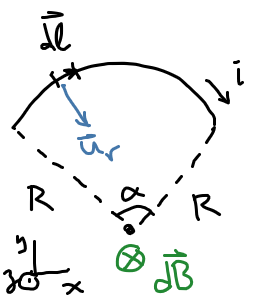
\includegraphics[scale=0.3]{08-champ-magnetique/figures/bs-champ-arc.png}
  \end{center}
}

Tous les petits morceaux du fil sont à la même distance du centre puisque c'est
un arc de cercle. L'angle entre $d\vec{l}$ et $\vu_r$ est toujours de
\SI{90}{\degree} parce que c'est un arc de cercle. Par la loi de Biot-Savart,
\begin{align*}
  d\vB &= \frac{\mu_0 i}{4\pi} \frac{d\vec{l} \times \vu_r}{r^2} \\
       &= \frac{\mu_0 i}{4\pi} \frac{dl \sin\theta (-\zhat)}{R^2} \\
       &= -\frac{\mu_0 i}{4\pi R^2} \zhat dl
\end{align*}
Par le principe de superposition, le champ total est obtenu en additionnant
les champs produits par tous les petits morceaux de fil:
\begin{align*}
  \vB &= \int_\mathrm{fil} -\frac{\mu_0 i}{4\pi R^2}\zhat dl  \\
      &= -\frac{\mu_0 i}{4\pi R^2}\zhat \int_\mathrm{fil} dl  \\
      &= -\frac{\mu_0 i}{4\pi R^2}\zhat R\alpha  \\
      &= -\frac{\mu_0 i \alpha}{4\pi R}\zhat
\end{align*}
On a intégré pour couvrir tout le fil, donc on obtient simplement longueur
totale du bout de fil.


\begin{diapobox}
  \subsection*{Machine d'imagerie par résonance magnétique}

  \marginnote{
    \footnotesize
    Aarnink, R. and Overweg, J. Magnetic Resonance Imaging a success story for
    superconductivity. Europhysics News, 43 4 (2012) 26-29. DOI:
    \url{https://doi.org/10.1051/epn/2012404}
  }
  Une machine d'imagerie par résonance magnétique permet de produire des images
  de l'intérieur du corps humain sans utiliser de technique invasive ni de
  rayonnement ionisant. Une machine typique produit un champ magnétique de
  \SI{1.50}{\tesla} au centre d'une bobine fait d'un supraconducteur
  (typiquement du nickel-titanium ou du nickel-étain). Si la bobine est faite
  de \num{10000} tours de fil et a un rayon de \SI{50}{\centi\meter}, quel est
  le courant qui doit circuler dans le fil?
\end{diapobox}

\begin{reponsebox}
  Calculons le champ magnétique d'une boucle de fil.
  \marginnote{
    \begin{center}
      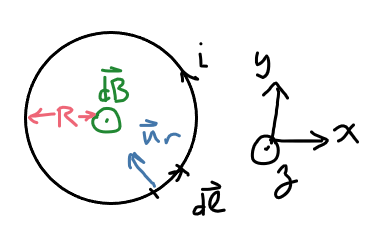
\includegraphics[scale=0.4]{08-champ-magnetique/figures/mri_figure_correcte.png}
    \end{center}
  }

  Tous les petits morceaux du fil sont à la même distance du centre puisque c'est
  un cercle. L'angle entre $d\vec{l}$ et $\vu_r$ est toujours de
  \SI{90}{\degree} parce que c'est un cercle. Par la loi de Biot-Savart,
  \begin{align*}
    d\vB_1 &= \frac{\mu_0 i}{4\pi} \frac{d\vec{l} \times \vu_r}{r^2} \\
         &= \frac{\mu_0 i}{4\pi R^2} \zhat dl
  \end{align*}
  Par le principe de superposition, le champ total est obtenu en additionnant
  les champs produits par tous les petits morceaux de fil:
  \begin{align*}
    \vB_1 &= \int_\mathrm{boucle} \frac{\mu_0 i}{4\pi R^2}\zhat dl  \\
        &= \frac{\mu_0 i}{4\pi R^2}\zhat \int_\mathrm{fil} dl  \\
        &= \frac{\mu_0 i}{4\pi R^2}\zhat 2\pi R  \\
        &= \frac{\mu_0 i}{2 R}\zhat
  \end{align*}
  On a intégré pour couvrir tout le fil, donc on obtient simplement longueur
  totale de la boucle. Chaque boucle génère un champ identique, donc le champ
  total, par le principe de superposition, est
  \begin{align*}
    \vB &= N\vB_1 \\
        &= \frac{\mu_0 i N}{2 R}\zhat
  \end{align*}
  Le champ total est connu, on cherche le courant donc
  \begin{align*}
    i &= \frac{2R B}{\mu_0 N}  \\
      &= \frac{2 \cdot \SI{50}{\centi\meter} \cdot \SI{1.5}{\tesla}}{4\pi
        \times 10^{-7} \cdot \num{10000}}  \\
      &= \SI{119.4}{\ampere}
  \end{align*}

  Si on utilisait du fil de cuivre de calibre 12 AWG
  (\SI{4}{\milli\meter\squared}), la résistance du fil serait de
  \begin{align*}
    R &= \frac{\rho \cdot 2 \pi R N}{A}  \\
      &= \SI{131.9}{\ohm}
  \end{align*}
  et la puissance dissipée dans le fil serait de
  \begin{align*}
    P &= Ri^2  \\
      &= \SI{1880}{\kilo\watt}
  \end{align*}
  C'est l'équivalent d'environ 450 cuisinières électriques qui fonctionnent à
  plein régime! De quoi faire des frites bien croustillantes!
\end{reponsebox}


\section{Champ magnétique d'un solénoïde}

\marginnote{
  Lafrance \S 8.6
}

Un solénoïde idéal est une succession de boucles de courant adjacentes formées
en enroulant un long fil autour d'un cylindre. On considère que le solénoïde a
une longueur infinie. Le champ magnétique peut être obtenu en appliquant le
principe de superposition pour additionner les champs produits par les boucles
individuelles. Le résultat est que le champ magnétique à l'extérieur du
solénoïde est nul et le champ magnétique à l'intérieur est uniforme et de
grandeur
$$B = \mu_0 i \frac{N}{L}$$
où $N/L$ est le nombre de tours par unité de longueur. La direction du champ
magnétique est obtenue en enroulant les doigts de la main droite dans la
direction du courant. Le pouce indique alors la direction du champ magnétique.


\begin{diapobox}
  Le réacteur à fusion nucléaire ITER est constitué d'une cavité toroïdale dans
  laquelle un plasma à haute température est confiné grâce à un champ
  magnétique de \SI{5.3}{\tesla}. Le champ magnétique est produit par un
  solénoïde toroïdal (un solénoïde dont les extrémités sont reliées ensembles).
  Le tore a un rayon d'environ \SI{6.2}{\meter} et les spires ont un rayon
  d'environ \SI{6.5}{\meter}. Le courant qui circule dans le câble est de
  \SI{68}{\kilo\ampere}. Quelle est la longueur de câble totale utilisée dans
  le solénoïde?
\end{diapobox}

\begin{reponsebox}
  Le nombre de ligne de champ par unité de longueur peut être obtenu par
  \begin{align*}
    B &= \mu_0 i n  \\
    n &= \frac{B}{\mu_0 i}  \\
      &= \SI{62.02}{\meter^{-1}}
  \end{align*}
  La longueur du solénoïde est
  \begin{align*}
    L &= 2\pi R  \\
      &= \SI{38.96}{\meter}
  \end{align*}
  où $R = \SI{6.2}{\meter}$. Le nombre total de tour est donc
  \begin{align*}
    N &= nL \\
      &= \frac{2\pi R B}{\mu_0 i}
  \end{align*}
  Chaque tour de câble a une longueur de $2\pi r$ où $r = \SI{6.5}{\meter}$. La
  longueur totale de câble est donc
  \begin{align*}
    d &= Nr  \\
      &= \frac{4\pi^2 rR B}{\mu_0 i}  \\
      &= \SI{98.68}{\kilo\meter}
  \end{align*}
\end{reponsebox}
